\section{Supplementary information}

\subsection{Locked protocol}\label{sec:protocol}
The confirmatory protocol (\texttt{docs/PREREGISTRATION\_v11.md}) fixed the cohorts, network,
tasks, training budget, learning-rate selection, conditions, endpoints, test families and
equivalence margin before any confirmation-cohort run. Its SHA-256, the source-code hash and the
analysis-script hash are recorded in \texttt{docs/LOCK\_v11.json} (Table~\ref{tab:lock}).

\begin{table}[h]\centering\small\caption{Protocol lock record.}\label{tab:lock}
\begin{tabular}{ll}\toprule
locked at utc & \texttt{2026-11-08T20:23:06.054737+00:00}\\
protocol sha256 & \texttt{34453091eb6167c1fcb563b9edb4ee73...}\\
source hash & \texttt{6f3ff264daccfdeee2dae6656539f3bf...}\\
analysis sha256 & \texttt{705004bdb741278852253c48243748dd...}\\
confirmation configs sha256 & \texttt{ecadfeb93d31af97f7390359925c76a1...}\\
\bottomrule\end{tabular}\end{table}


\subsection{Connection-probability prior}
\begin{table}[h]\centering\small
\caption{Type-level connection probabilities $P(\text{target}\leftarrow\text{source})$ used to
draw the recurrent mask. They are modelling assumptions inspired by
\citet{pfeffer2013,pi2013}, not measurements for the sampled cells.}\label{tab:priors}
\begin{tabular}{lcccc}\toprule
target $\backslash$ source & Pyr & PV & SST & VIP\\ \midrule
Pyr & 0.20 & 0.50 & 0.45 & 0.05\\
PV  & 0.45 & 0.35 & 0.30 & 0.05\\
SST & 0.35 & 0.05 & 0.05 & 0.70\\
VIP & 0.30 & 0.05 & 0.40 & 0.05\\ \bottomrule
\end{tabular}\end{table}

\subsection{Selected learning rates}
\begin{table}[h]\centering\small
\caption{Learning rates selected on the development cohort by validation BCE (recurrent / readout). The frozen reservoir has no recurrent rate.}\label{tab:lr}
\begin{tabular}{llcccc}\toprule
task & optimizer & BPTT & local & local (no $\beta$) & reservoir\\ \midrule
early & adam & 0.001 / 1 & 0.003 / 3 & 0.001 / 3 & -- / 3\\
early & rms & 0.001 / 10 & 0.003 / 0.3 & 0.0003 / 0.3 & -- / 0.3\\
late & adam & 0.003 / 1 & 0.001 / 3 & 0.001 / 1 & -- / 3\\
late & rms & 0.003 / 3 & 0.001 / 1 & 0.003 / 0.3 & -- / 0.3\\
dms & adam & 0.003 / 1 & 0.003 / 1 & 0.001 / 1 & -- / 3\\
dms & rms & 0.003 / 0.1 & 0.001 / 1 & 0.003 / 0.3 & -- / 0.3\\
\bottomrule\end{tabular}\end{table}


\subsection{Supplementary figures}
\begin{figure}[h]\centering
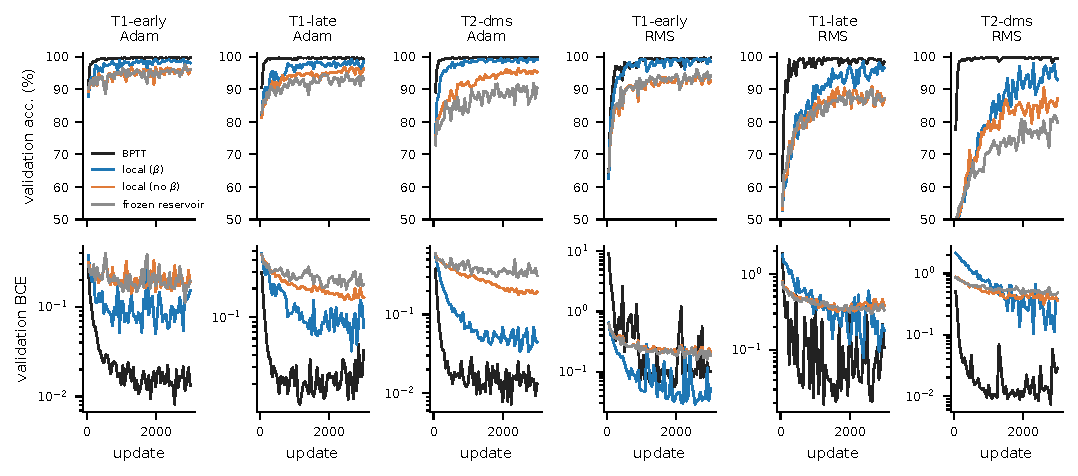
\includegraphics[width=\textwidth]{figures/figS1_learning_curves.pdf}
\caption{\textbf{Validation learning curves} (in-distribution trials; mean over 16 confirmation
networks) for each learner, task and optimizer. Accuracy saturates early, and validation BCE keeps
falling for all learners.}\label{fig:s1}
\end{figure}
\begin{figure}[h]\centering
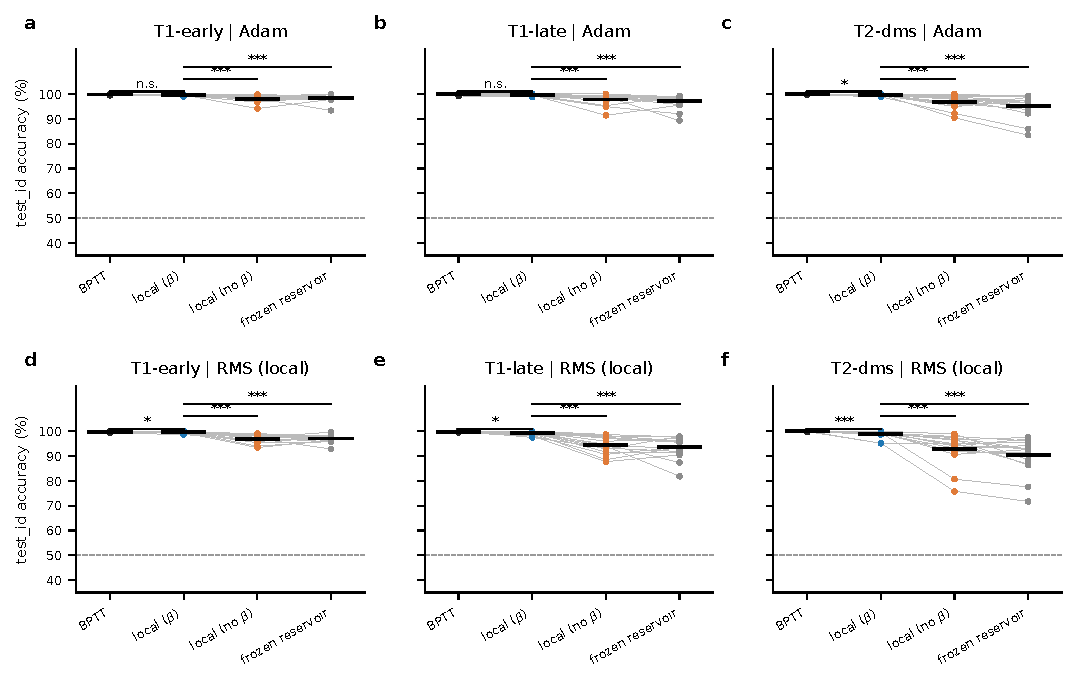
\includegraphics[width=\textwidth]{figures/figS2_id_accuracy.pdf}
\caption{\textbf{In-distribution accuracy} (training delays) for the learners of
Fig.~\ref{fig:rules}. Every learner is near ceiling, which is why the preregistered endpoint uses
unseen delays. Brackets show the same contrasts on this secondary endpoint (Holm within that
endpoint).}\label{fig:s2}
\end{figure}

\subsection{Relation to earlier versions of this project}
Earlier internal versions compared intact and shuffled cells while keeping the intact bank's
calibration. They split cells by specimen (65 donors were shared between cohorts), compared
learners after a fixed short budget at which none had converged, and used one task. Those
results are not used here. All numbers in this paper come from the runs described in
Methods.
